\documentclass[platex,dvipdfmx]{jsarticle}
\usepackage{amsmath}
\usepackage{amssymb}
\usepackage{algorithm}
\usepackage{algorithmic}
\usepackage{graphicx}
\usepackage[table]{xcolor}
\usepackage{listings}

\title{マルチメディア信号処理 第1回レポート課題}
\author{28G17038河野達彦\\28G17041 小寺健太}

\textheight 25cm
\topmargin -2cm
\textwidth 16cm
\oddsidemargin 0cm

\begin{document}
  
\maketitle

\section{課題1.1}
\subsection{アルゴリズム概要}
私たちの班はC++で以下のようなプログラムを作成した.

\begin{algorithm}                      
\caption{拡大・縮小・回転に対応するパターンマッチング}         
\label{alg1}                          
\begin{algorithmic}                  
\REQUIRE テンプレート画像10〜15枚,探索対象画像(image.pgm)
\ENSURE 各テンプレート画像の中心位置座標,拡大倍率,回転角
\STATE 画像の読み込み
\FOR {image.pgmを左上からスキャン} 
  \IF {画素が黒でない}
    \STATE target $\leftarrow$ 8近傍で接続しているオブジェクトを切り抜く
    \FOR {各テンプレート画像に対して}
      \STATE オブジェクトの画素値の合計から各テンプレートの拡大倍率を算出
      \FOR {回転角= -90 to 90}
        \STATE template $\leftarrow$ 拡大倍率と回転角を反映したテンプレート画像を用意し切り抜く
        \STATE diff $\leftarrow (\mbox{target}と\mbox{template}の画素値の差)^2 の和 / 比較画素数$
      \ENDFOR
    \ENDFOR
    \STATE targetに対して最小のdiffを与えるtemplate番号,中心位置座標,拡大倍率,回転角を出力
  \ENDIF
\ENDFOR
\end{algorithmic}
\end{algorithm}

\subsection{実装の詳細}
\subsubsection{画像の読み込み}
画像に関するデータをメンバにもつクラスを用意し,
そのメソッドとしてReaddata()を作成した.
Readdata()はファイルパスを引数とし,bool値を返す.
メソッド内で画素値データを2次元vectorのdataに格納し,
またその画素値が走査済みかどうかを保持する2次元vectorのvisitedを作成する(makevisited()).
与えられたpgmファイルは画像の幅や高さ,各画素値はスペース区切りで羅列されている.
よってifstreamで画像を開いたのち>>演算子を用いることでうまく読み込みができた.
template画像の番号は連続であるがフォルダによって画像の数が異なるため,
ファイルの取得に失敗した場合はfalseを返す関数として実装し
全てのtemplate画像を読み込むようにした.\\

  
\begin{lstlisting}[basicstyle=\ttfamily\footnotesize, frame=single]

  // 画像の読み込み ファイルが存在しない場合false を返す
  bool readdata(string filename){
    string str;
    ifstream fin(filename);
    if(fin){
      fin >> str; fin.ignore();
      if(str != "P2") cout << "file format error" << endl;
      getline(fin, str); // コメント読み捨て
      fin >> W >> H; 
      data.resize(H);
      for(int i=0; i<H; i++){
        data[i].resize(W);
      }
      fin >> str; //255
      int h=0, w=0;
      while(fin >> str){
        data[h][w] = stoi(str);
        w  = (w+1) % W;
        if(w == 0) h++; 
      }
      makevisited();
      return true;
    }
    else return false;
  }

   \end{lstlisting}
\newpage


\subsubsection{画像の切り抜き}
Algorithm1において切り抜きと表現した操作はtrimming()メソッドによって行われる.
trimming()は黒でない画素座標を引数とし,8近傍で連結するオブジェクトに内接する長方形を考え
その左上点の座標と長方形の幅および高さを計算する.
それに加え拡大倍率算出に使われるオブジェクトの画素値の合計も同時に計算する.
連結部の走査はQueueを用いた幅優先探索アルゴリズムで実現した.
これに伴い,画素値が走査済みかどうかを保持する2次元vectorであるvisitedが必要になる.
visitedの要素はboolであり,Raddata()内で黒でない画素が格納されている座標にfalseを格納した.
1度訪れた画素座標にはtrueが格納される.\\

  \begin{lstlisting}[basicstyle=\ttfamily\footnotesize, frame=single]

  // 未踏はfalse, 訪問済みtrue
  // 0が入っている場所はtrue, ついでに総面積S(=画素値の合計)も算出
  void makevisited(){
    visited.resize(H);
    for(int i=0; i<H; i++){
      visited[i].assign(W,false);
    }
    S = 0;
    for(int h=0; h<H; h++){
      for(int w=0; w<W; w++){
        if(data[h][w] == 0){
          visited[h][w] = true;
        }
        else{
          S += data[h][w];
        }
      }
    }
  }


  // 内接する四角の左上端と幅,オブジェクトの画素値の合計を計算
  void trimming(int h, int w){
    queue<Point> que;
    int dp[3] = {-1,0,1};
    que.push({h,w});
    visited[h][w] = true; 
    S_trim = data[h][w];
    int max_h=0, min_h=MAX, max_w=0, min_w=MAX;
    while(que.size()){
      Point p = que.front(); que.pop();
      max_h = max(max_h, p.h);
      min_h = min(min_h, p.h);
      max_w = max(max_w, p.w);
      min_w = min(min_w, p.w);
      for(int i=0; i<3; i++){
        for(int j=0; j<3; j++){
          Point np = {p.h + dp[i], p.w + dp[j]};
          if(np.h>=0 && np.h<H && np.w>=0 && np.w<W){
            if(! visited[np.h][np.w]){
              que.push(np);
              S_trim += data[np.h][np.w];
              visited[np.h][np.w] = true;
            }
          }
        }
      }
    }
    upleft.h = min_h;
    upleft.w = min_w;
    H_trim = max_h - min_h;
    W_trim = max_w - min_w;
  }

     \end{lstlisting}

\newpage

\subsubsection{ノイズ処理}
ノイズが非常に多い画像に対するマッチング処理を行うため,ノイズ除去を行う関数を実装した.
ノイズ部分は白か黒,すなわち画素値は$0 or 255$であるため,この二種類の値を取っている画素について処理を行うことでノイズ除去による情報量の減少を抑えようと考えた.
周辺8近傍の平均値がしきい値を上回った・下回った場合にはそれぞれ画素値を$0,255$とする実装を行った.
また,我々のパターンマッチングのアイディアは黒でないピクセルから,隣接する白でない画素をなぞることで画像を切り抜くが,この切り抜いた部分の大きさが小さかった場合はノイズと判断する様に実装したため周辺が黒い部分での白のノイズの除去は一定の成果が出た時点で完成とした.
  \begin{lstlisting}[basicstyle=\ttfamily\footnotesize, frame=single]

  	// 画素情報と周辺平均を投げると条件によってノイズの画素を綺麗にする
	void remove_noise_pixel(vector<vector<int>>& nonoise_data,
    int h,int w,int peripheral_ave){
		if(data[h][w] == 0 && 
        peripheral_ave > REMOVE_NOISE_WHITE_THRESHOLD){
			nonoise_data[h][w] = 255;
		}
		else if(data[h][w] == 255 && peripheral_ave < REMOVE_NOISE_BLACK_THRESHOLD){
			nonoise_data[h][w] = 0;
		}else{
			nonoise_data[h][w] = data[h][w];
		}
	
	}

}

  // ノイズ除去
  void remove_noise(){
    int peripheral_ave = 0;

    vector<vector<int>> nonoise_data;
    nonoise_data.resize(H);
    for(int i=0; i<H; i++){
      nonoise_data[i].resize(W);
    }
    
    for(int h=0; h<H; h++){
      for(int w=0; w<W; w++){
        // 四辺上の端は周辺1画素ずつは取れない(はみ出す)ので対策
        if(h == 0){
          // 上辺
          if(w==0){
            peripheral_ave = (data[h][w+1] + data[h+1][w] + data[h+1][w+1]) / 3;
          }
          if(w==W){
            peripheral_ave = (data[h][w-1] + data[h+1][w-1] + data[h+1][w]) / 3;
          }else{
            peripheral_ave = (data[h][w-1] + data[h][w+1] + data[h+1][w-1] 
            + data[h+1][w] + data[h+1][w+1]) / 5;
          }
          remove_noise_pixel(nonoise_data,h,w,peripheral_ave);
        }else if(h == H-1){
          // 下辺
          if(w==0){
            peripheral_ave = (data[h-1][w] + data[h-1][w+1] + data[h][w+1]) / 3;
          }
          if(w==W){
            peripheral_ave = (data[h-1][w-1] + data[h-1][w] + data[h][w-1]) / 3;
          }else{
            peripheral_ave = (data[h-1][w-1] + data[h-1][w] + data[h-1][w+1] 
            + data[h][w-1] + data[h][w+1]) / 5;
          }
          remove_noise_pixel(nonoise_data,h,w,peripheral_ave);
        }else if(w == 0){
          // 左辺
          peripheral_ave = (data[h-1][w] + data[h-1][w+1] + data[h][w+1] 
          + data[h+1][w] + data[h+1][w+1]) / 5;
          remove_noise_pixel(nonoise_data,h,w,peripheral_ave);
        }else if(w == W-1){
          // 右辺
          peripheral_ave = (data[h-1][w-1] + data[h-1][w] + data[h][w-1]
           + data[h+1][w-1] + data[h+1][w]) / 5;
          remove_noise_pixel(nonoise_data,h,w,peripheral_ave);
        }
        // 隣接周辺画素がすべて取れるエリア
        else if(data[h][w] == 0){
          // 黒画素
          peripheral_ave = (data[h-1][w-1] + data[h-1][w] + data[h-1][w+1] 
          + data[h][w-1] + data[h][w+1] + data[h+1][w-1] + data[h+1][w] 
          + data[h+1][w+1]) / 8;
          if(count_black(h,w) < 4){
            nonoise_data[h][w] = 255;
          }else if(peripheral_ave > REMOVE_NOISE_WHITE_THRESHOLD){
            nonoise_data[h][w] = 255;
          }else{
            nonoise_data[h][w] = data[h][w];
          }
        }else if(data[h][w] == 255){
          // 白画素
          peripheral_ave = (data[h-1][w-1] + data[h-1][w] + data[h-1][w+1]
           + data[h][w-1] + data[h][w+1] + data[h+1][w-1] + data[h+1][w] 
           + data[h+1][w+1]) / 8;
          if(count_white(h,w) < 4){
            nonoise_data[h][w] = 0;
          }else if(peripheral_ave < REMOVE_NOISE_BLACK_THRESHOLD){
            nonoise_data[h][w] = 0;
          }else{
            nonoise_data[h][w] = data[h][w];
          }
        }else{
          nonoise_data[h][w] = data[h][w];
        }
      }
    }
    data = nonoise_data;
  }

  \end{lstlisting}


\newpage

\subsubsection{拡大倍率と回転への対応}
実装当初は画素数の比を元にtemplate画像の拡大倍率を算出していたが良い結果が得られなかった.
某氏の助言により画素値の総和の比を元に算出したところ非常に良い精度で得られた.
image.pgm中の注目しているオブジェクトに対して切り出しを行なっているため画素値の総和は既知である.
さらに各template画像についても読み込み時に既に算出している.
したがって総当たりをすることなく,各template画像が注目オブジェクトに
一致するとしたときの拡大倍率を算出することが可能である.
一方,回転については-90度〜90度の180通りを総当たりした.

\subsubsection{targetとtemplateの比較方法}
今回の課題において要となるのはimage.pgm中の注目しているオブジェクト(target)と
拡大倍率,回転角を反映した各種template画像(template)を何を基準にして比較するかという点だろう.
本プログラムではtargetとtemplateの両方に対して内接する長方形で切り出しを行うことで解決した.
もしtargetに対して適切なtemplate画像,拡大倍率,回転角のtemplateであれば,
切り出した後の画像は等しくなるはずである.
したがって単純に左上のピクセルから比較すればよいことが分かる.
この手法を実現するためにはtemplateの画像データを用意し切り出しを行う必要がある.
balance()関数はあるtemplate元画像クラス,拡大倍率,回転角を引数とし,
それらを反映した新たなtemplate画像クラスを返す関数である.
なお生成する画像は特に補完を行わず,写像後小数点以下を切り捨てた画素値を与えた.\\

   
\begin{lstlisting}[basicstyle=\ttfamily\footnotesize, frame=single]

// 入力画像をscale倍しrot度回転させた画像を返す
Image balance(Image templates, double scale, int rot){
    double theta = rot*M_PI/180;
    Image temp;
    temp.H = templates.H * scale;
    temp.W = templates.W * scale;
    // 28*28のオリジナルtemplate画像から画素を持ってくるので拡大倍率によらず中心は常に(14,14)
    Point c = {templates.H/2, templates.W/2};

    temp.data.resize(temp.H);
    for(int i=0; i<temp.H; i++)
      temp.data[i].resize(temp.W);

    //画像中心を中心として回転
    for(int h=0; h<temp.H; h++){
      for(int w=0; w<temp.W; w++){
        double h_s = h/scale;
        double w_s = w/scale;
        int h_r = cos(-theta)*(h_s-c.h) - sin(-theta)*(w_s-c.w) + c.h;
        int w_r = sin(-theta)*(h_s-c.h) + cos(-theta)*(w_s-c.w) + c.w;
        if(h_r >= templates.H) h_r = templates.H-1;
        if(w_r >= templates.W) w_r = templates.W-1;
        if(h_r < 0) h_r = 0;
        if(w_r < 0) w_r = 0;
        temp.data[h][w] = templates.data[h_r][w_r];
      }
    }
    temp.makevisited();
    return temp;
}

\end{lstlisting}



また比較の範囲はtargetとtemplateが重なっている部分のみとした.
これは切り出し後の幅と高さについて2画像のの最小値をとることで実現できる.
targetと最も一致するtemplateは,1画素あたりの画素値の差の2乗が最小のものとした.
某氏の指摘により比較領域の画素数で割ることに気づき精度が向上したことを記しておく.
\newpage


\subsubsection{特徴点抽出}
手書きの数値画像の特徴点として,以下の項目が使えると考えた.
\begin{itemize}
	\item{画素値の合計}
	\item{画素値の上下の偏り}
	\item{画素値の左右の偏り}
\end{itemize}
画素値の合計とは,画像の画素の値を合計しただけのものである.
単純な値ではあるが,文字の面積を図ることが出来るので特徴点として利用可能だと考えた.
これはマッチング処理にて既に実装していた為,そのまま利用した.

また,画素値が左右,上下でどれくらい偏ってるかによって上下対照・左右対称等の特徴を反映できるのではないかと考え,実装し実験を行った.

\newpage
\subsection{実行環境と結果}
以下はMacbook Pro(Intel~Corei5~2GHzプロセッサ,8GBメモリ)で実行した結果である.
また実行時間はchornoライブラリを用いて計測した.
なおコンパイルは g++ ~-O3~-std=c++11~で行った.

\subsubsection{image1}
\begin{figure}[h]
\centering
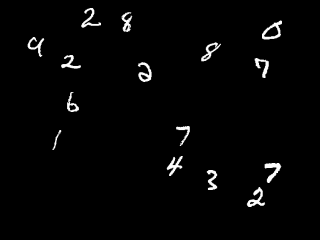
\includegraphics[clip,width = 8.5cm]{images/image1.png}
\caption{image1~ 解答と実行結果}
\label{graph1}
\end{figure}

\begin{table}[]
\centering
\caption{image1~実行結果と解答}
\label{my-label1}
\begin{tabular}{|l|l|l|l|l||l|l|l|l|l|}
\hline
\multicolumn{5}{|c||}{解答}          & \multicolumn{5}{c|}{実行結果}             \\ \hline
画像         & w   & h   & 回転角 & 拡大倍率 & 画像         & w   & h   & 回転角 & 拡大倍率 \\ \hline
template1  & 212 & 179 & 0   & 1    & template1  & 212 & 179 & 0   & 1    \\ \hline
template2  & 145 & 72  & 0   & 1    & template2  & 145 & 72  & 0   & 1    \\ \hline
template3  & 126 & 22  & 0   & 1    & template3  & 126 & 22  & 0   & 1    \\ \hline
template4  & 70  & 63  & 0   & 1    & template4  & 70  & 63  & 0   & 1    \\ \hline
template5  & 36  & 45  & 0   & 1    & template5  & 36  & 45  & 0   & 1    \\ \hline
template6  & 56  & 139 & 0   & 1    & template6  & 56  & 139 & 0   & 1    \\ \hline
template7  & 184 & 132 & 0   & 1    & template7  & 184 & 132 & 0   & 1    \\ \hline
template8  & 262 & 66  & 0   & 1    & template8  & 262 & 66  & 0   & 1    \\ \hline
template9  & 71  & 104 & 0   & 1    & template9  & 71  & 104 & 0   & 1    \\ \hline
template10 & 272 & 170 & 0   & 1    & template10 & 272 & 170 & 0   & 1    \\ \hline
template11 & 209 & 51  & 0   & 1    & template11 & 209 & 51  & 0   & 1    \\ \hline
template12 & 272 & 31  & 0   & 1    & template12 & 272 & 31  & 0   & 1    \\ \hline
template13 & 256 & 198 & 0   & 1    & template13 & 256 & 198 & 0   & 1    \\ \hline
template14 & 174 & 165 & 0   & 1    & template14 & 174 & 165 & 0   & 1    \\ \hline
template15 & 89  & 19  & 0   & 1    & template15 & 89  & 19  & 0   & 1    \\ \hline
\end{tabular}
\end{table}
実行時間は1.351秒であった.
座標,回転角,拡大倍率の全てを正しく得ることができた.

\subsubsection{image2}
\begin{figure}[h]
\centering
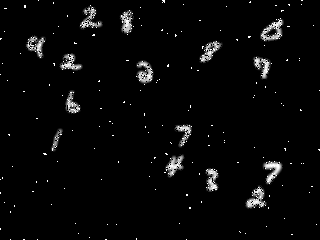
\includegraphics[clip,width = 8.5cm]{images/image2.png}
\caption{image2~ ノイズ除去後の画像}
\label{graph2}
\end{figure}

\begin{table}[]
\centering
\caption{image1~実行結果と解答}
\label{my-label1}
\begin{tabular}{|l|l|l|l|l||l|l|l|l|l|}
\hline
\multicolumn{5}{|c||}{解答}          & \multicolumn{5}{c|}{実行結果}             \\ \hline
画像         & w   & h   & 回転角 & 拡大倍率 & 画像         & w   & h   & 回転角 & 拡大倍率 \\ \hline
\rowcolor[HTML]{C0C0C0}
template1	&212	&179	&0	&1& template13	& 174	&	165&	0&	1 \\ \hline
\rowcolor[HTML]{C0C0C0}
template2	&145	&72	&0	&1& template2 	& 85 	&	14 &	0&	1 \\ \hline
template3	&126	&22	&0	&1& template3 	& 127	&	20 &	0&	1 \\ \hline
\rowcolor[HTML]{C0C0C0}
template4	&70	&63	&0	&1& template4 	& 265	&	28 &	0&	1 \\ \hline
template5	&36	&45	&0	&1& template5 	& 34 	&	43 &	0&	1 \\ \hline
\rowcolor[HTML]{C0C0C0}
template6	&56	&139	&0	&1& template6 	& 208	&	48 &	0&	1 \\ \hline
\rowcolor[HTML]{C0C0C0}
template7	&184	&132	&0	&1& template7 	& 63 	&	62 &	0&	1 \\ \hline
template8	&262	&66	&0	&1& template8 	& 260	&	62 &	0&	1 \\ \hline
\rowcolor[HTML]{C0C0C0}
template9	&71	&104	&0	&1& template9 	& 144	&	68 &	0&	1 \\ \hline
\rowcolor[HTML]{C0C0C0}
template10	&272	&170	&0	&1& template10	& 69 	&	102&	0&	1 \\ \hline
\rowcolor[HTML]{C0C0C0}
template11	&209	&51	&0	&1& template11	& 182	&	131&	0&	1 \\ \hline
\rowcolor[HTML]{C0C0C0}
template12	&272	&31	&0	&1& template12	& 58 	&	137&	0&	1 \\ \hline
template13	&256	&198	&0	&1& template13	& 253	&	194&	0&	1 \\ \hline
\rowcolor[HTML]{C0C0C0}
template14	&174	&165	&0	&1& template14	& 272	&	172&	0&	1 \\ \hline
\rowcolor[HTML]{C0C0C0}
template15	&89	&19	&0	&1& template15	& 212	&	177&	0&	1 \\ \hline
\end{tabular}
\end{table}

実行時間は40ミリ秒であった.\\
なお,この課題のみ回転角と拡大倍率は固定とした.
template3,5,8,13以外は全て誤認識となった.

\subsubsection{image3}
\begin{figure}[h]
\centering
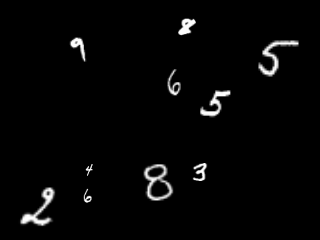
\includegraphics[clip,width = 8.5cm]{images/image3.png}
\caption{image3~ 回答と実行結果}
\label{graph3}
\end{figure}

% Please add the following required packages to your document preamble:
% \usepackage[table,xcdraw]{xcolor}
% If you use beamer only pass "xcolor=table" option, i.e. \documentclass[xcolor=table]{beamer}
\begin{table}[]
\centering
\caption{image3~ 解答と実行結果}
\label{my-label3}
\begin{tabular}{|l|l|l|l|l||l|l|l|l|l|}
\hline
\multicolumn{5}{|c||}{解答}            & \multicolumn{5}{c|}{実行結果}               \\ \hline
画像         & w   & h   & 回転角 & 拡大倍率 & 画像         & w   & h   & 回転角 & 拡大倍率     \\ \hline
template1  & 40  & 209 & 0   & 1.9  & template1  & 38  & 207 & -1  & 1.89766  \\ \hline
\rowcolor[HTML]{C0C0C0} 
template2  & 87  & 197 & 0   & 0.7  & template8  & 86  & 196 & -18 & 0.820375 \\ \hline
template3  & 157 & 181 & 0   & 1.8  & template3  & 156 & 180 & 3   & 1.79956  \\ \hline
template4  & 89  & 169 & 0   & 0.6  & template4  & 88  & 169 & 0   & 0.599469 \\ \hline
template5  & 78  & 45  & 0   & 1.2  & template5  & 76  & 43  & 3   & 1.20264  \\ \hline
template6  & 186 & 26  & 0   & 0.9  & template6  & 185 & 25  & 0   & 0.896784 \\ \hline
template7  & 214 & 104 & 0   & 1.5  & template7  & 212 & 102 & -2  & 1.4978   \\ \hline
template8  & 173 & 85  & 0   & 1.3  & template8  & 172 & 84  & -2  & 1.30326  \\ \hline
template9  & 275 & 55  & 0   & 2    & template9  & 274 & 54  & -2  & 2.00127  \\ \hline
template10 & 200 & 171 & 0   & 0.9  & template10 & 199 & 170 & -3  & 0.898823 \\ \hline
\end{tabular}
\end{table}


\newpage
実行時間は0.879秒であった.
template2がtemplate8と誤識別されてしまった.
他のオブジェクトに関しては座標は2以内,拡大倍率は0.01以内,
回転角は3度以内の誤差で検出できた.
\newpage


\subsubsection{image4}

\begin{figure}[h]
\centering
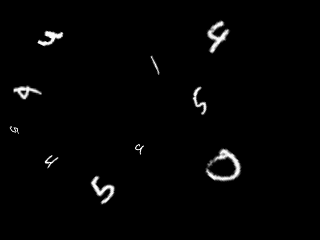
\includegraphics[clip,width = 8.5cm]{images/image4.png}
\caption{image4}
\label{graph4}
\end{figure}

\begin{table}[]
\centering
\caption{image4~解答と実行結果}
\label{my-label4}
\begin{tabular}{|l|l|l|l|l||l|l|l|l|l|}
\hline
\multicolumn{5}{|c||}{解答}            & \multicolumn{5}{c|}{実行結果}               \\ \hline
template番号 & w   & h   & 回転角 & 拡大倍率 & template番号 & w   & h   & 回転角 & 拡大倍率     \\ \hline
template1  & 217 & 36  & -35 & 1.6  & template1  & 216 & 34  & -33 & 1.59986  \\ \hline
template2  & 50  & 37  & 65  & 1    & template2  & 48  & 36  & 65  & 0.999354 \\ \hline
template3  & 225 & 165 & -38 & 1.6  & template3  & 224 & 163 & -37 & 1.6004   \\ \hline
template4  & 50  & 161 & -8  & 0.7  & template4  & 49  & 160 & -9  & 0.698452 \\ \hline
template5  & 139 & 148 & -11 & 0.5  & template5  & 137 & 147 & -22 & 0.498287 \\ \hline
template6  & 25  & 91  & 87  & 1.4  & template6  & 23  & 91  & 87  & 1.39994  \\ \hline
template7  & 14  & 129 & -69 & 0.5  & template7  & 13  & 128 & -78 & 0.49995  \\ \hline
template8  & 155 & 64  & 29  & 1    & template8  & 154 & 63  & 29  & 1        \\ \hline
template9  & 199 & 101 & 55  & 1.1  & template9  & 197 & 100 & 53  & 1.09943  \\ \hline
template10 & 102 & 190 & 44  & 1.3  & template10 & 100 & 189 & 41  & 1.29979  \\ \hline
\end{tabular}
\end{table}
\newpage
実行時間は0.769秒であった.
全てのオブジェクトに関して十分な精度で検出できた.
座標は2以内,拡大倍率は0.01以内,回転角は11度以内の誤差で検出できた.

\newpage

\subsubsection{image5}
\begin{figure}[h]
\centering
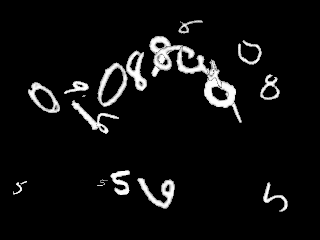
\includegraphics[clip,width = 8.5cm]{images/image5.png}
\caption{image5}
\label{graph5}
\end{figure}
20個のうち正しく識別できたのはtemplate7,8,9,12,17,20の6個であった.
オブジェクト同士が重なっている画像を識別することは今後への課題とする.

\newpage

\subsubsection{特徴点抽出}

書いてある数字によって偏りが出ている.これらのパラメーターは手書き文字の判別に利用が可能だと考えられる.
\begin{figure}[h]
\centering
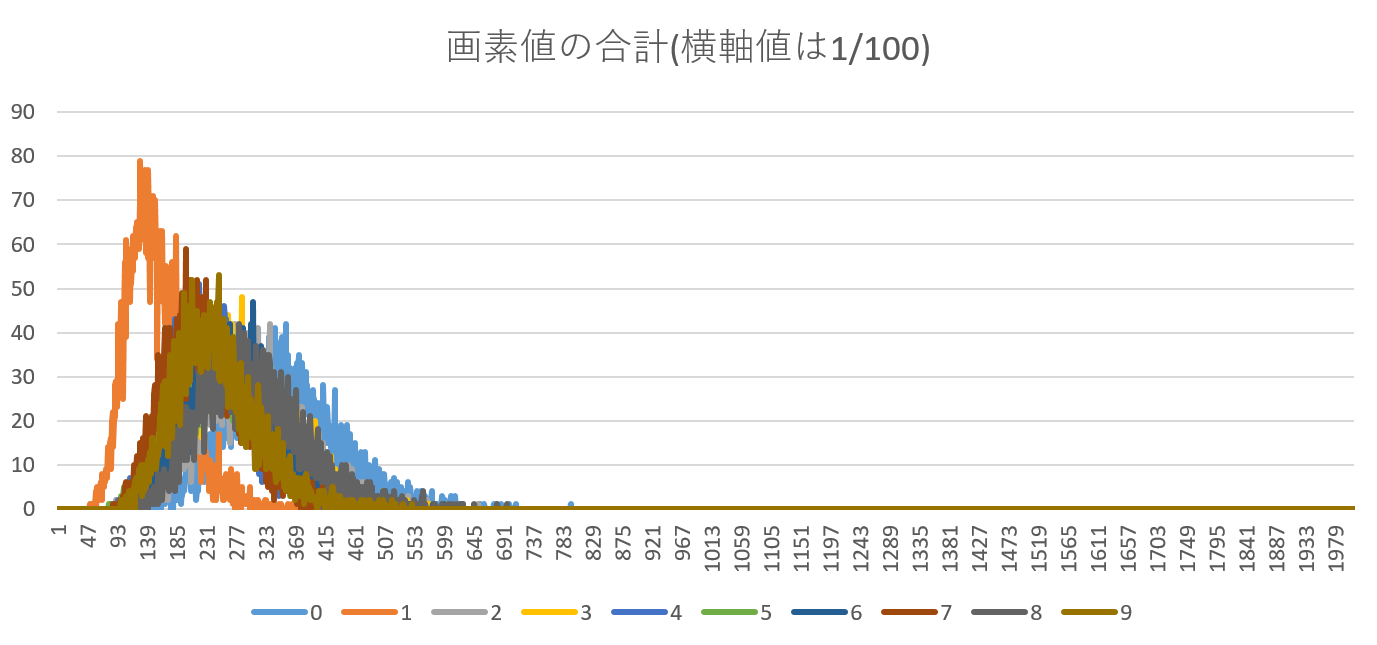
\includegraphics[width = 11.5cm]{images/graph/summation.PNG}
\caption{画素値の合計}
\label{summation}
\end{figure}

\begin{figure}[h]
\centering
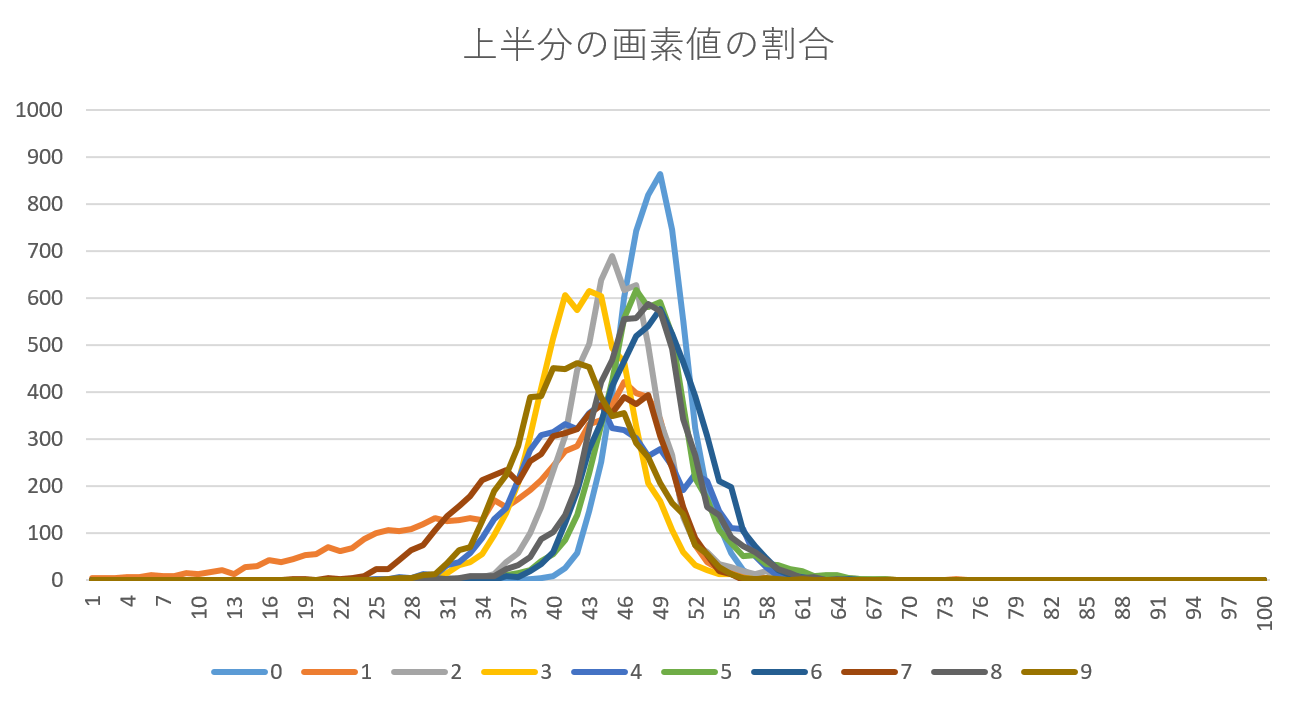
\includegraphics[width = 11.5cm]{images/graph/upper.PNG}
\caption{上半分の画素値の合計}
\label{upper}
\end{figure}

\begin{figure}[h]
\centering
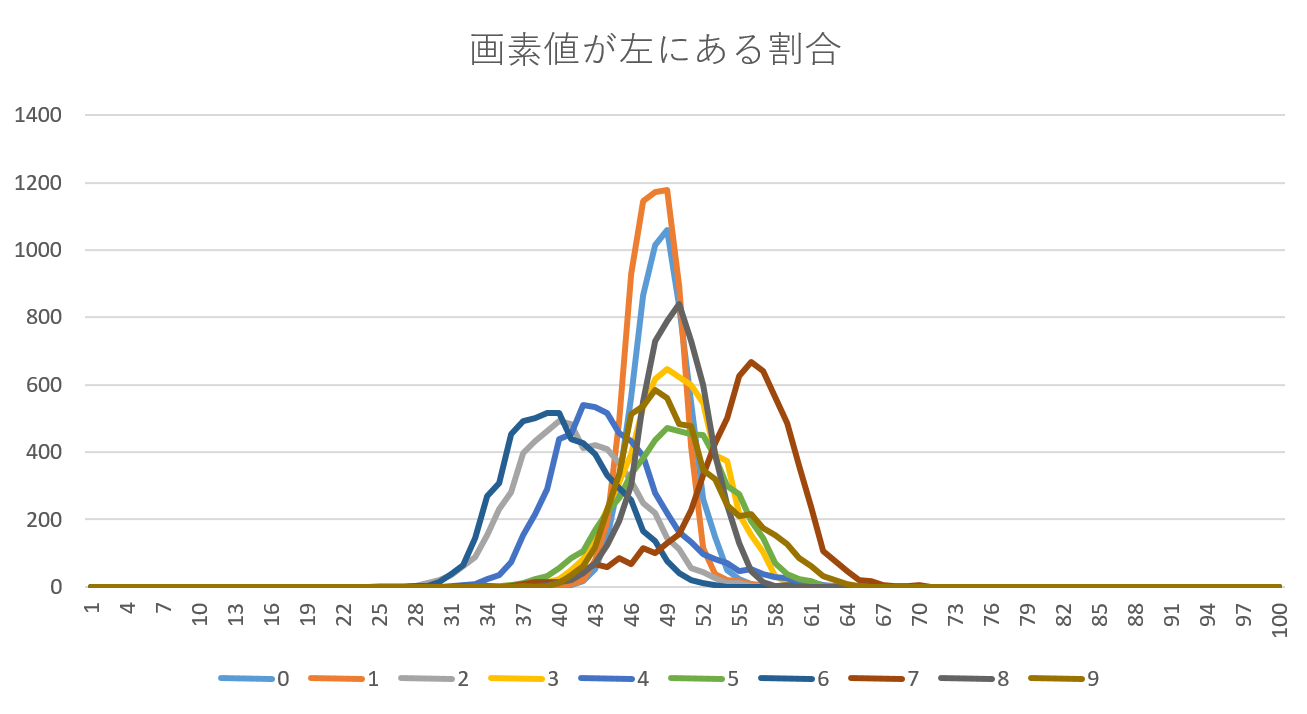
\includegraphics[width = 11.5cm]{images/graph/left.PNG}
\caption{左半分の画素値の合計}
\label{left}
\end{figure}

\subsection{考察}
\subsubsection{計算時間}
全ての拡大倍率,回転角について総当たりをした場合の計算量は,
image.pgmの高さと幅$H, W$, template画像の高さと幅$H_t, W_t$,
拡大倍率$S$, 回転角$R$, template画像数$T$を用いて
\begin{align*}
  O(H \cdot W \cdot H_t \cdot W_t \cdot S \cdot R \cdot T)
\end{align*}
で表される.これはおよそ$10^{13}$ステップあり
全テンプレートの走査に10000秒程度かかることが予想される.\\
一方今回私たちのプログラムは以下の計算量で走査を終える.
\begin{align*}
  O(H \cdot W + H_t \cdot W_t + H_t \cdot W_t \cdot  R \cdot T \cdot T)
\end{align*}
これはおよそ$10^8$ステップあり,1/10秒ほどで全テンプレートの走査を終えることができると考えられる.
上記の実験では1秒前後で終えることができ,明らかな改善があったと言える.

\subsubsection{精度}
image3における誤識別や,出力結果の誤差について考察する.
図5はimage.pgm中のオブジェクトと本アルゴリズムで作られたtemplate画像である.

\begin{figure}[htbp]
\begin{center}
  \begin{tabular}{c}

    % 1枚目の画像
    \begin{minipage}{0.5\hsize}
      \begin{center}
        
\includegraphics[clip, width=60mm]{images/naoko.png}
        \hspace{1.6cm} (a)image.pgm中のオブジェクト
      \end{center}
    \end{minipage}

    % 2枚目の画像
    \begin{minipage}{0.5\hsize}
      \begin{center}
        
\includegraphics[clip, width=60mm]{images/trimming.png}
        \hspace{1.6cm} (b)template画像に拡大・回転処理をした画像
      \end{center}
    \end{minipage}

  \end{tabular}
  \caption{}
  \label{fig:img}
  \end{center}
\end{figure}

このように明らかな補完処理の差があるため,
特に違いの少ない手書き文字の識別は非常に難しくなる.

\newpage

\section{感想}
\subsection{河野}
僕自身がC++でのコードの実装,また論理的にアルゴリズムを考えて実装するといった事には慣れていなかったため,
チームメイトである小寺君へのアドバイスをする余裕があまりなく,予定より全体的に手間取ってしまった.
カプセル化や関数切り分けのポイント等を指示するなど,互いの経験値になることを考えていたが課題の処理に負われてしまったのは反省点である.
だが,この課題のコードを作りっぱなしにせず提出後も一部修正を加える予定であるのでそれを通じて僕もプログラミングのレベルアップを図りたいと考えている.

\subsection{小寺}
河野さんがメインで実装を行うと簡単にできてしまいそうだったので,
僕の実装をサポートをしていただくお願いを聞き入れてもらった.
複雑ではないプログラムとはいえ,1から実装するのは思ったよりも苦労した.
今回の課題で最大の山場はtargetとtemplateを比較する方法である.
重心を使わずにできないかと考え,思いついた時は非常に嬉しかった.
また画像の回転を実装する際,あくまでtemplateの元画像から画素値を参照しているために
画像の中心位置は拡大倍率によらない点に気付くまで苦労した.
加えて,あらかじめ引数をそのまま返す関数を書いておき後ほど拡張したり,
可読性を上げるために名前が短く分かりやすい変数を新たに宣言したりといった,
ただ結果を出すだけでなく今後に繋がるような学びが多くあった.
様々な角度で的確な助言をくれた河野さん並びに西田くんには非常に感謝している.
まだまだ直すところはたくさんありそうなので,今後も修正を続けたい.


\section*{付録}
\begin{lstlisting}[basicstyle=\ttfamily\footnotesize, frame=single]

// g++ -O3 -std=c++11 find.cpp && ./a.out
#include <iostream>
#include <fstream>
#include <vector>
#include <string>
#include <queue>
#include <cmath>
#include <chrono>
using namespace std;

typedef struct{
  int h;
  int w;
}Point;

typedef struct{
  int template_num;
  int diff;
  Point c_dist;
  double scale;
  int rot;
}Output;

class Image{
public:
  const int MAX = 10000;
  int W, H, W_trim, H_trim;
  double S, S_trim;
  Point upleft;
  vector<vector<int>> data;
  vector<vector<bool>> visited;

  // 画像の読み込み ファイルが存在しない場合falseを返す
  bool readdata(string filename){
    string str;
    ifstream fin(filename);
    if(fin){
      fin >> str; fin.ignore();
      if(str != "P2") cout << "file format error" << endl;
      getline(fin, str); // コメント読み捨て
      fin >> W >> H; 
      data.resize(H);
      for(int i=0; i<H; i++){
        data[i].resize(W);
      }
      fin >> str; //255
      int h=0, w=0;
      while(fin >> str){
        data[h][w] = stoi(str);
        w  = (w+1) % W;
        if(w == 0) h++; 
      }
      makevisited();
      return true;
    }
    else return false;
  }

  // 未踏はfalse, 訪問済みtrue
  // 0が入っている場所はtrue, ついでに総面積S(=画素値の合計)も算出
  void makevisited(){
    visited.resize(H);
    for(int i=0; i<H; i++){
      visited[i].assign(W,false);
    }
    S = 0;
    for(int h=0; h<H; h++){
      for(int w=0; w<W; w++){
        if(data[h][w] == 0){
          visited[h][w] = true;
        }
        else{
          S += data[h][w];
        }
      }
    }
  }

  // 内接する四角の左上端と幅,オブジェクトの画素値の合計を計算
  void trimming(int h, int w){
    queue<Point> que;
    int dp[3] = {-1,0,1};
    que.push({h,w});
    visited[h][w] = true; 
    S_trim = data[h][w];
    int max_h=0, min_h=MAX, max_w=0, min_w=MAX;
    while(que.size()){
      Point p = que.front(); que.pop();
      max_h = max(max_h, p.h);
      min_h = min(min_h, p.h);
      max_w = max(max_w, p.w);
      min_w = min(min_w, p.w);
      for(int i=0; i<3; i++){
        for(int j=0; j<3; j++){
          Point np = {p.h + dp[i], p.w + dp[j]};
          if(np.h>=0 && np.h<H && np.w>=0 && np.w<W){
            if(! visited[np.h][np.w]){
              que.push(np);
              S_trim += data[np.h][np.w];
              visited[np.h][np.w] = true;
            }
          }
        }
      }
    }
    upleft.h = min_h;
    upleft.w = min_w;
    H_trim = max_h - min_h;
    W_trim = max_w - min_w;
  }
};

// 入力画像をscale倍しrot度回転させた画像を返す
Image balance(Image templates, double scale, int rot){
    double theta = rot*M_PI/180;
    Image temp;
    temp.H = templates.H * scale;
    temp.W = templates.W * scale;
    // 28*28のオリジナルtemplate画像から画素を持ってくるので拡大倍率によらず中心は常に(14,14)
    Point c = {templates.H/2, templates.W/2};

    temp.data.resize(temp.H);
    for(int i=0; i<temp.H; i++)
      temp.data[i].resize(temp.W);

    //画像中心を中心として回転
    for(int h=0; h<temp.H; h++){
      for(int w=0; w<temp.W; w++){
        double h_s = h/scale;
        double w_s = w/scale;
        int h_r = cos(-theta)*(h_s-c.h) - sin(-theta)*(w_s-c.w) + c.h;
        int w_r = sin(-theta)*(h_s-c.h) + cos(-theta)*(w_s-c.w) + c.w;
        if(h_r >= templates.H) h_r = templates.H-1;
        if(w_r >= templates.W) w_r = templates.W-1;
        if(h_r < 0) h_r = 0;
        if(w_r < 0) w_r = 0;
        temp.data[h][w] = templates.data[h_r][w_r];
      }
    }
    temp.makevisited();
    return temp;
}

int main(){
  // 時間計測開始


  Image target;
  target.readdata("images/images4/image.pgm");
  
  // template画像がある限り読み込み
  vector<Image> templates;
  for(int i=0; 1;i++){
    templates.resize(i+1);
    if(! templates[i].readdata("images/images4/template"+to_string(i+1)+".pgm")){
      templates.resize(i);
      break;
    }
  }
  auto start = std::chrono::system_clock::now();
  // targetの走査 オブジェクトを見つけるごとに最適なtemplateを探す
  for(int h=0; h<target.H; h++){
    for(int w=0; w<target.W; w++){
      if(! target.visited[h][w]){
        target.trimming(h,w);
        Output ans;
        ans.diff = 2147483647;
        Output now;
        for(int i=0; i<templates.size(); i++){
          now.template_num = i;
          // templateの倍率を画素値の和の比から求め,角度は-90~90まで総当たり
          now.scale = sqrt((double)target.S_trim / (double)templates[i].S);
          for(int r=0; r<180; r++){
            now.rot = r-90;
            Image temp = balance(templates[i], now.scale, now.rot);
            // templateは1度trimmingできればよい 縮小により離れた点を読むことを防ぐ
            bool trimmed = false;
            for(int h_=0; h_<temp.H; h_++){
              for(int w_=0; w_<temp.W; w_++){
                if(! temp.visited[h_][w_] and ! trimmed){
                  temp.trimming(h_, w_);
                  now.c_dist = {temp.H/2-temp.upleft.h, temp.W/2-temp.upleft.w};
                  trimmed = true;
                }
              }
            }
            // 左上の点を合わせて比較   範囲は小さい方に合わせる
            int diff = 0;
            Point range = {min(target.H_trim,temp.H_trim), min(target.W_trim, temp.W_trim)};
            for(int dh=0; dh<range.h; dh++){
              for(int dw=0; dw<range.w; dw++){
                int temp_pixel = temp.data[temp.upleft.h+dh][temp.upleft.w+dw];
                int target_pixel = target.data[target.upleft.h+dh][target.upleft.w+dw];
                // 1画素あたりの画素値の差の2乗を求める
                diff += pow((temp_pixel - target_pixel), 2) / (range.h * range.w) ;
              }
            }
            // diffが小さい方を答えとする
            if(diff < ans.diff){  
              now.diff = diff;  
              ans = now;
            }
          }
        }
        int center_h = target.upleft.h + (ans.c_dist.h);
        int center_w = target.upleft.w + (ans.c_dist.w);
        cout << "template" << ans.template_num+1 << "  " << center_w << "  " << center_h 
             << " " << ans.rot << "  " << ans.scale << endl;
        ofstream ofs("result.csv",ios::app);
        ofs << "template" << ans.template_num+1 << "," << center_w << "," << center_h 
             << "," << ans.rot << "," << ans.scale << endl;
      }
    }
  }

  auto end = std::chrono::system_clock::now();     
  auto dur = end - start;       
  auto msec = std::chrono::duration_cast<std::chrono::milliseconds>(dur).count();
  std::cout << msec << " milli sec \n";
  return 0;
}


\end{lstlisting}

\end{document}

